\documentclass[11pt]{amsart}
\usepackage{geometry}                % See geometry.pdf to learn the layout options. There are lots.
\geometry{letterpaper}                   % ... or a4paper or a5paper or ...
%\geometry{landscape}                % Activate for for rotated page geometry
%\usepackage[parfill]{parskip}    % Activate to begin paragraphs with an empty line rather than an indent
\usepackage{booktabs}
\usepackage{graphicx}
\usepackage{amssymb}
\usepackage{epstopdf}
\usepackage{caption}
\usepackage{subcaption}
\usepackage{commath}
\DeclareGraphicsRule{.tif}{png}{.png}{`convert #1 `dirname #1`/`basename #1 .tif`.png}

% Declare commands
\newcommand{\mat}[1]{\mathbf{#1}}

\title{CS 181 -- Practical 3}
\author{Casey Grun, Sam Kim, Rhed Shi}
%\date{}                                           % Activate to display a given date or no date

\begin{document}
\maketitle

% -----------------------------------------------------------------------------
\section{Warmup}


% -----------------------------------------------------------------------------
\section{Classification}

Our challenge was to classify a set of programs, based on traces of their system calls, as either a type of malware or a non-malicious program. Given an $N \times D$ matrix $\mat{X}$ representing the programs, along with a $N$-dimensional vector $\vec{t}$ of training labels, produce a function 
$$y : \mat{X'} \mapsto \vec{t'}$$.
That is, a function which could produce labels $\vec{t'}$ for some matrix $\mat{X'}$. There were two parts to this challenge: determining the \emph{feature functions} to generate rows of the matrix $\mat{X}$ based on the system calls for each malware program, and determining what classification algorithm to use to generate the function $y$.

We developed a cross-validation procedure to test our predictions on folds of the training data before submitting our predictions to Kaggle on the test data; we used 10 folds. A persistent problem we observed was that predicted scores in cross-validation were 0.1--0.2 higher than the scores we recieved on the public leaderboard on Kaggle. We suspect this was because of the heterogeneous training data 

\subsection{Feature Functions}

We evaluated a number of feature functions:
\begin{description}
  \item[System call counts] Our first feature simply summed the number of system calls across all threads in all processes for a particular program. This method achieved ???? on the public leaderboard.
  \item[$n$-grams of system calls] Our most substantial feature examined counts of sequences of system calls. Each unique sequence of $n$ system calls was represented as a feature that counted how many times this sequence appeared in any given malware. We used cross-validation to try and optimize the choice of $n$---the length of these sequences. Too small an $n$ would result in uninformative sequences, while too large an $n$ would not generalize well. We found the optimum $n$ to be approximately 8. 
  \item[DLLs loaded] We also created features counting how many times each unique DLL was loaded with the \verb|load_dll| system call. This feature proved to be reasonably informative, and achieved our best score on Kaggle (in combination with the 8-grams of system calls). 
  \item[Registry keys] Finally, we employed a similar method to count the number of times each unique registry key was read by a program. This feature was less informative than the DLLs or 8-grams, so it was not included in our final predictions.
\end{description}

Additionally, we attemped classification on a reduced-dimensionality feature set, generated by performing a truncated singular value decomposition (TSVD) on the full feature set. This method did not perform particularly well, so it was not pursued. 

Our final/best score was achieved by combining the DLLs, 8-grams, and system call counts features.

\begin{figure}
  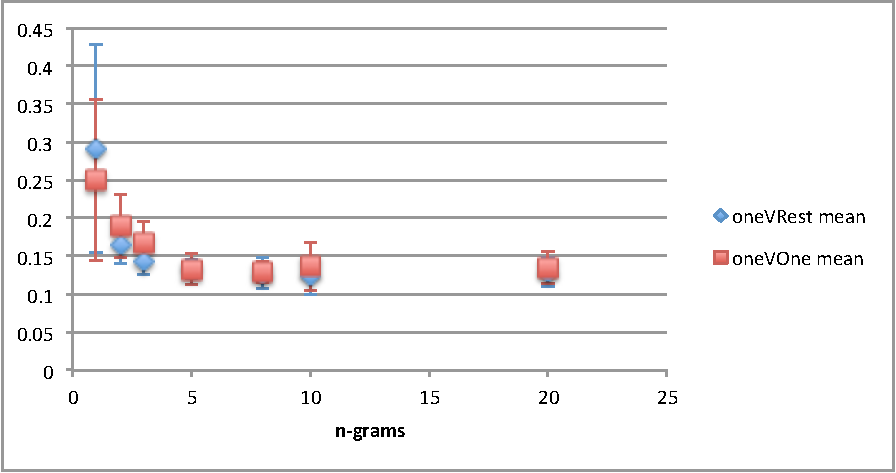
\includegraphics{n-grams.pdf}
  \caption{Tuning the length $n$ of sequences of system calls. Y-axis is error.}
\end{figure}

\begin{figure}
  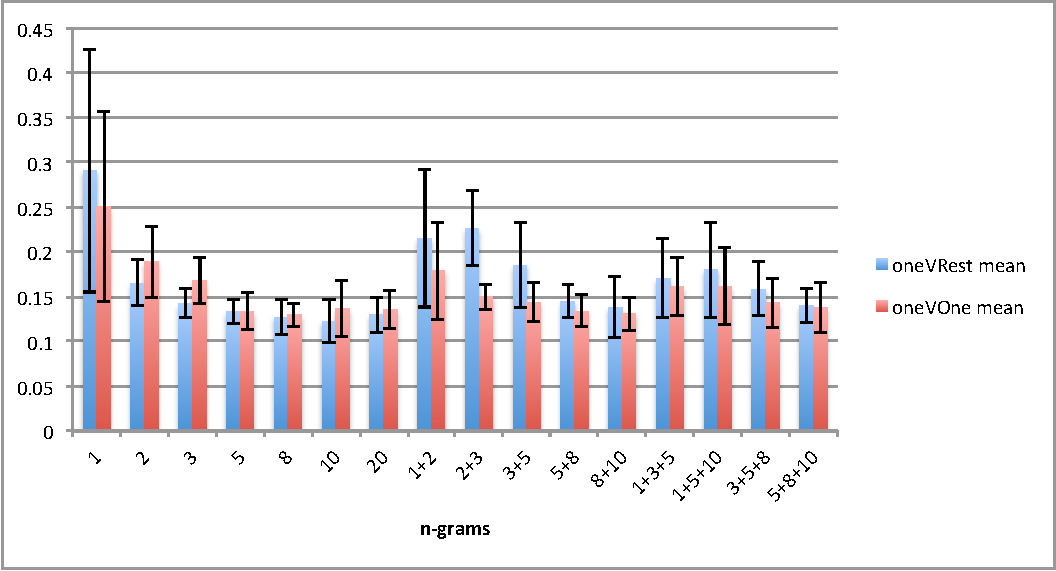
\includegraphics{n-grams-combos.pdf}
  \caption{Considering combinations of $n$-grams of system calls. Y-axis is error.}
\end{figure}

\begin{figure}
  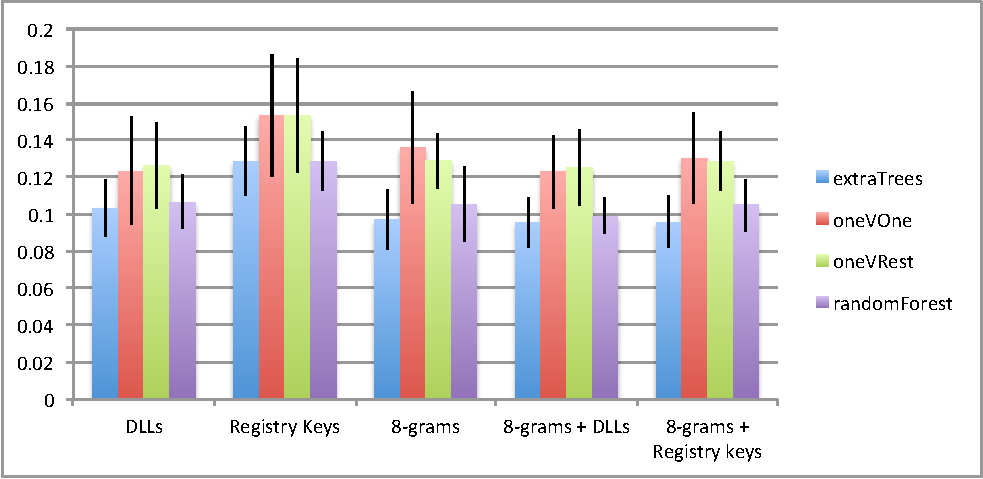
\includegraphics{other_features.pdf}
  \caption{Comparison of best-performing features. Y-axis is error.}
\end{figure}

\begin{figure}
  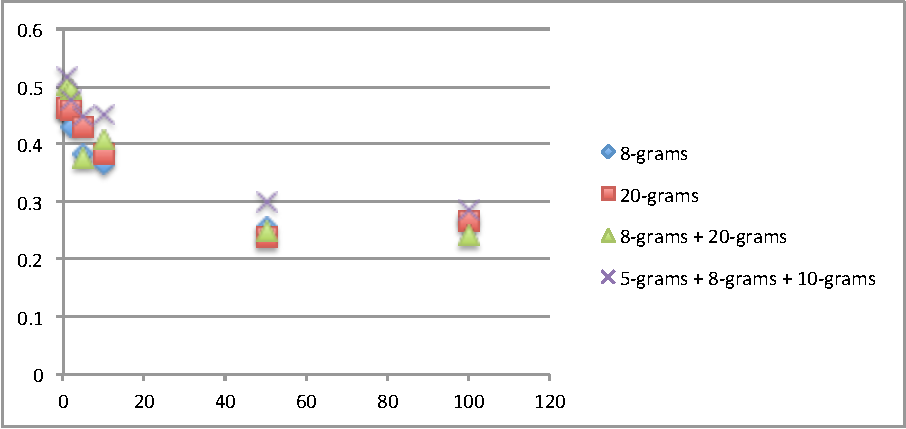
\includegraphics{tsvd.pdf}
  \caption{Comparison of a truncated singular value decomposition (TSVD) on various combinations of $n$-grams. The TSVD performed considerably worse than the full feature set in cross-validation, so it was not pursued.}
\end{figure}


\subsection{Classification Methods}
We evaluated a number of classification learning algorithms, as implemented by the scikit-learn Python library. These include:
\begin{description}
  \item[One-vs-rest] As discussed in the textbook, this algorithm fits one classifier per class to classify if a point is in a class $C_k$ or not. We used linear discriminant functions.
  \item[One-Vs-One] This algorithm introduces a discriminant function for every pair of classes, where each point is classified according to a majority of decisions among the discriminant functions. We used linear discriminant functions.
  \item[Logistic regression] This algorithm minimizes an error based on the training set to optimize the parameters for the likelihood function.
  \item[Decision trees] This algorithm goes down a tree of binary nodes in which the inputs are used to determine which path to go down, which ultimately assign probabilities to the target variable.
  \item[Forests of randomized trees] Related to the decision trees, this algorithm uses a set of trees, where each tree is built using random decisions. Whereas a decision tree will use the best split among all the features for each node, the random tree will pick the best split from a random subset of features. The trees are built independently and then their results are averaged to make predictions. This results in the bias increasing (due to not picking the best split) but the variance decreasing (due to averaging) which offsets the increase in bias.
  \item[Forests of extremely randomized trees] This is similar to the forests of randomized trees algorithm, except that splits are computed slightly differently in building the random trees. In addition to using a random subset of features for each node, instead of picking the best feature, thresholds are drawn randomly for each feature and these thresholds are picked as the splitting rules. This results in an even higher bias but lower variance.
\end{description}

We evaluated these learning algorithms based on the extracted features of system call counts and system call bigrams, and using cross-validation methods to withhold 10\% of the data over 10 trials and averaging the percent errors over the predictions on the withheld data. Standard deviations over the 10 trials were calculated and the average running time for a single learning and prediction run are also noted. The results are summarized in the table below:\\

\begin{tabular}{l | r | l | l}
Classification algorithm & \% error & Standard deviation & Running time (s)\\
\hline
One-vs-rest (linear) & 12.7 & 2.4 & 7-8 \\
One-vs-one (linear) & 12.9 & 1.4 & 7-9\\
Logistic regression & 11.5 & 1.5 & 600-700\\
Decision tree & 10.9 & 1.3 & 50-60 \\
Random trees & 10.4 & 1.2 & 8-10\\
Extremely random trees & 9.7 & 1.6 &16-20\\
\end{tabular}
\\
\\
Additionally, on Kaggle, the one-vs-rest, decision tree, and extremely random trees classification algorithms using the system call counts and system call bigrams reached accuracies of 68.5\%, 79.1\%, and 81.0\%, respectively.\\


% -----------------------------------------------------------------------------
\section{Conclusion}


% -----------------------------------------------------------------------------
\begingroup
\begin{thebibliography}{9}

%\bibitem{LSMR}
%Fong, David Chin-Lung, and Michael Saunders. "LSMR: An iterative algorithm for sparse least-squares problems."
%\emph{SIAM Journal on Scientific Computing} 33.5 (2011): 2950-2971

\end{thebibliography}
\endgroup

\end{document}